
\section{Main Ideas}
\label{s:mainIdeas}
As a warm up and to introduce some notation and ideas, we first describe a simple algorithm that produces a hypergraph from a graph by including every possible hyperedge. This can result in a hypergraph that has many more hyperedges than the maximum \emph{a posteriori} (MAP) hypergraph, and therefore has far lower posterior probability. Correspondingly, this simple algorithm succeeds in a smaller range of edge densities than the MAP rule, however, this algorithm does turn out to succeed in a nontrivial parameter range. We then describe our algorithm for constructing the MAP hypergraph and the associated guarantees.

% \gb{Check if there's a better name -- what do they call it in empirical paper?}
\subsection{Maximum Clique Cover Algorithm}
\label{sec:maxclique}
When the graph is so sparse that each hyperedge appears as an isolated clique, exact recovery is easily achieved by creating a hypergraph with a hyperedge for every clique of the projected graph $\pG$. This algorithm turns out to succeed far beyond the regime where hyperedges do not overlap.
% \cg{This might be a good place to introduce the clique graph}


Let the \emph{$d$-clique hypergraph }$\cliG$ of the projected graph $\pG=([n], E_p)$ be the hypergraph $\cliG = ([n],\cliE=\cli(\pE))$ where
\[
\cli(E) = \b\{\he\in \textstyle{\binom{[n]}{d}} : (i,j)\in E
\text{ for every } \{i,j\}\subset h
\b\}\,.
\]
% We use $\Ic(\he)$ to be the indicator that a hyperedge $\he$ is included in $\cliG$.
% It is easy to see that any $\hE\in \prim(E)$ is a subset of $\cli(E)$. 
% \cg{cg: only retain what is really used below}
% Notice that there is a bijection between all possible $d$-clique hypergraphs and the image set of $\proj$, as $\proj(\cli(E))=E$. 
% When we say the minimum preimage or the minimum cover of a $d-$clique hypergraph, we refer to the minimum preimage or the minimum cover of the corresponding projected graph.
% 
Denote by $\cliA$ the algorithm converting every size-$d$ clique in $\pG $ to a hyperedge in the output graph, i.e., $\cliA(\pG) = \cli(\pE)$. We call this the \emph{maximum clique cover algorithm}.

% \begin{algorithm}\caption{Maximum Clique Cover Algorithm $\cliA$}\label{alg:clique-cover}
% \begin{algorithmic}[1]
% \STATE Input: $\pG = ([n],\pE)$
% \STATE  $\cli(\pE)\leftarrow \emptyset$
% \FOR{all size $d$ subsets of $[n]$}
%     \STATE If $\pE$ has a clique on the subset, add the hyperedge on the subset to $\cli(\pE)$
% \ENDFOR
% \STATE Output $\cli(\pE)$
% \end{algorithmic}
% \end{algorithm}

\begin{algorithm}\caption{Maximum Clique Cover Algorithm $\cliA$}\label{alg:clique-cover}
\begin{algorithmic}[1]
\State Input: $\pG = ([n],\pE)$
\State  $\cli(\pE)\leftarrow \emptyset$
\For {all size $d$ subsets of $[n]$}
    \State If $\pE$ has a clique on the subset, add the hyperedge on the subset to $\cli(\pE)$
\EndFor
\State Output $\cli(\pE)$
\end{algorithmic}
\end{algorithm}

\begin{remark}
    Since we are enumerating all size-$d$ subsets, the algorithm has time complexity $n^d$. It may be possible to improve this runtime by taking advantage of sparsity of the graph, using ideas in \cite{boix2021average}. 
\end{remark}


For which parameters does this algorithm work? 
% Unfortunately, this does not reach the optimal threshold. 
From the definition, $\cliA$ fails if and only if there exists a clique in $\pG$ that is not a hyperedge of $\rhG$. 
If a $d$-clique $\he$ in $\pG$ is not a hyperedge of $\rhG$, every edge in the clique is included in some other hyperedge $\he'\in \rhG$. By carefully examining the possible ways of inclusion for all edges, we can obtain a tight bound on the probability of the event, yielding the following threshold.

% \gbdone{why is this $d-1$ in denom while Theorem 1.3 has $d$?}
% \cg{It should be $d$, this is a typo.}
\begin{theorem}\label{thm:naive}
    $\cliA$ exactly recovers $\rhG$ when $\delta< \frac{d-3}{d}$ and has $\Omega_n(1)$ probability of failure when $\delta\ge \frac{d-3}{d}$.
\end{theorem}
This implies the positive recovery  result in Theorem~\ref{thm:main-large-d} for $d\geq 6$, which we believe to be suboptimal. The proof of Theorem~\ref{thm:naive} is in Appendix~\ref{sec:naive}. 
% 


\subsection{Greedy Algorithm}
Another natural algorithm starts with the maximum clique cover algorithm and then greedily deletes redundant hyperedges from the clique graph.


\begin{algorithm}\caption{Greedy Algorithm}\label{alg:greedy}
\begin{algorithmic}[1]
\State Input: $\pG = ([n],\pE)$
\State Find the $d$-clique hypergraph $H_0\leftarrow\cli(\pE)$
\While{$\exists h\in H_0$ that $H_0\backslash h\in \proj^{-1}(\hE_\rhG)$}
    \State $H_0\leftarrow H_0\backslash h$
\EndWhile
\State Output $H_0$
\end{algorithmic}
\end{algorithm}

% \begin{algorithm}\caption{Greedy Algorithm}\label{alg:greedy}
% \begin{algorithmic}[1]
% \STATE Input: $\pG = ([n],\pE)$
% \STATE Find the $d$-clique hypergraph $H_0\leftarrow\cli(\pE)$
% \WHILE{$\exists h\in H_0$ that $H_0\backslash h\in \proj^{-1}(\hE_\rhG)$}
%     \STATE $H_0\leftarrow H_0\backslash h$
% \ENDWHILE
% \STATE Output $H_0$
% \end{algorithmic}
% \end{algorithm}

% \begin{enumerate}
%     \item Find the $d$-clique hypergraph $H_0\leftarrow\cli(\pE)$.
%     \item Delete a hyperedge from $H_0$ if after the deletion the graph is still in $\proj^{-1}(\hE_\rhG)$. Repeat until all hyperedge cannot be deleted.
%     \item Output $H_0$
% \end{enumerate}

Heuristically this algorithm ought to work better than the maximum clique cover algorithm, because it yields a graph with higher posterior probability. We leave it as an open question to determine under which parameter regime this algorithm succeeds. 
% \cg{Is there more we can say this algorithm? An alternative choice is to put this in open problem session.}

\subsection{Information-Theoretically Optimal Algorithm: MAP}


% \nbyp{I think it is absolutely crucial to discuss here the clique cover stuff. I.e. define Algo 1 which just declares all cliques as hyperedges and state Theorem for its performance. Than Algo 2 which reports minimal clique cover as a hypergraph and say that this is MAP and its what we use for the lower bound on delta.}

Although fully determining the landscape of exact recovery is non-trivial, the optimal algorithm for the task is in fact not hard to describe. 
Given the projected graph $\pG = \proj(\rhG)$, the error probability upon outputting $\cA(\pG)$ is simply the complement of the probability that our guess was the true hypergraph,
\[
1-p_{\rhG|\pG}(\cA(\pG)|\pG) \,.
\]
Here $p_{\rhG|\pG}$ is the conditional probability mass function of the random hypergraph given the projected graph.
Therefore, if we do not worry about time complexity, the information theoretically optimal algorithm should simply output a hypergraph with maximum posterior likelihood, i.e., following the maximum \emph{a posteriori} (MAP) rule. As discussed next, the MAP rule can be easily characterized.

\paragraph{MAP Outputs a Minimum Preimage.}

Since the posterior distribution is
\[
p_{\rhG|\pG}(H|\pG) =\frac{\ind{\proj(\hE_H) = \pE}p_{\rhG}(\hE_H) }{p_\pG(\pE)}\propto  \ind{\proj(\hE_H) = \pE} \b(\frac{p}{1-p}\b)^{|\hE_H|}\,,
\]
the optimal algorithm $\cA^*$ should output one of the hypergraphs that project to $\pG$ with the smallest number of hyperedges, i.e., 
\[
\cA^*(\pG) \in \argmin_{\hG:\hE_{\hG}\in \prim(\pE)} |\hE_{\hG}|\,.
\]We say a hypergraph $\hG$ is 
% a \emph{preimage} of a graph $G=(V,E)$ if $\hE_\hG\in \prim(E)$ and is 
a \emph{minimum preimage} if $\hG\in \argmin_{\hE_\hG\in \prim(E)} |\hE_{\hG}|$. 


Since ties can be broken arbitrarily, we always assume that $\cA^*$ chooses a specific minimum preimage (for instance based on lexicographical order on the hyperedges) instead of choosing a random one.
% \footnote{\cg{State the optimality of MAP as a lemma?}}

% Some terminology will be useful. 


% \red{
% \begin{itemize}
%     \item Break down the optimal algorithm in terms of 2-connected components
%     \item Threshold for the branching of 2-connected components, explain why this branching process is non-trivial, as it is affected by "fake" hyperedges. 
%     \item Below the threshold, we only need to look at small subgraphs
%     \item Two theorems that states $\cdel d$ is only controlled by the appearance of "graph of two minimum preimages". Maybe a name for such graph?
% \end{itemize}
% }

\subsection{MAP is Efficient for Sparse Graphs}

In general, the MAP algorithm involves solving for the minimum way to cover a graph with a hypergraph, which can be intractable. In this section, we will provide an efficient algorithm for computing the MAP rule if the hypergraph is sparse enough, of course also making use of the fact that the hypergraph is random.
\begin{theorem}\label{thm:sparse-algo}
    When $\delta<\frac{d-1}{d+1}$, the optimal algorithm $\cA^*$ is with high probability efficiently computable (i.e., has runtime polynomial in $n$).
\end{theorem}
The underlying intuition is that when the hypergraph is sparse enough, we can partition the projected graph into constant-size components, where the minimum preimage of each component can be solved for independently of the other components. However, a naive definition of connected component is useless, as $p$ is far above the connectivity threshold. We require a definition of component better suited to our goal of finding the minimum preimage.



\paragraph{2-Neighborhood and 2-Connectivity.}



Define the \emph{2-neighbor} of a hyperedge $\he$ in a hypergraph $\hG$ to be all hyperedges $\he'$ with $|\he\cap \he'|\ge 2$, denoted by 
\[
\nei{\hG}(\he) = \{\he':|\he\cap \he'|\ge 2\}\,.
\]
Let $\mathcal{G}_\hG$ be a graph whose node set is the set of hyperedges in $\hG$ and the neighborhood structure is defined by 2-neighbors. We say that a set of hyperedges in $\hG$ is \emph{2-connected} if they are connected in $\mathcal{G}_\hG$. A \emph{2-connected component} of the hypergraph $\hG$ is a set of hyperedges that form a connected component in $\mathcal{G}_\hG$.\footnote{Here the definition is for hypergraphs and is different from the usual definition of 2-connectivity in a simple graph. }
See an illustration of 2-connectivity in Figure~\ref{fig:2-connectivity}. 
We will never need to refer to the graph $\mathcal{G}_\hG$ and instead work directly with 2-connected sets of hyperedges in $H$. 
% \gbdone{Is this true? }

% \begin{figure}
% \begin{subfigure}[\textwidth]
%     \centering\begin{tikzpicture}[every node/.style={fill,circle,inner sep=1.5pt},scale=0.8]

% \end{tikzpicture}
% \end{subfigure}

% \begin{subfigure}[\textwidth]
    
% \begin{tikzpicture}
% node at (0,0);
% \end{tikzpicture}
% \end{subfigure}

% \end{figure}

% \begin{figure}
% \begin{minipage}{0.48\textwidth}\centering
%     \begin{tikzpicture}[every node/.style={fill,circle,inner sep=1.5pt},yscale=0.9,xscale=0.8]

%   % Define the coordinates for the shared vertices of orange triangles
%   \coordinate (P1) at (0,0);
%   \coordinate (P2) at (2,0);
%   \coordinate (P3) at (1,1.732); % height of equilateral triangle
%   \coordinate (P4) at (3,1.732);

%   % Draw the orange triangles
%   \filldraw[orange, fill=orange!20] (P1) -- (P2) -- (P3) -- cycle; % 1st triangle
%   \filldraw[orange, fill=orange!20] (P2) -- (P3) -- (P4) -- cycle; % 2nd triangle
%   \coordinate (P5) at (4,0); % Shift for the 3rd triangle
%   \filldraw[orange, fill=orange!20] (P2) -- (P4) -- (P5) -- cycle; % 3rd triangle
%   \coordinate (P6) at (5,1.732); % Height for the 4th triangle
%   \filldraw[orange, fill=orange!20] (P4) -- (P5) -- (P6) -- cycle; % 4th triangle
%   \coordinate (P7) at (1,-1.732);
%   \filldraw[orange, fill=orange!20] (P1) -- (P2) --(P7) -- cycle;

%   % Define the coordinates for the red triangles
%   \coordinate (R1) at (5,-1.732);
%   \coordinate (R2) at (6,0); 
%   \coordinate (R3) at (7,-1.732);

%   % Draw the red triangles
%   \filldraw[red, fill=red!20] (P5) -- (R1) -- (R2) -- cycle; % 1st red triangle
%   \filldraw[red, fill=red!20] (R2) -- (R1) -- (R3) -- cycle; % 2nd red triangle

%   % The 3rd red triangle
%   \coordinate (R4) at (8,0);
%   \filldraw[red, fill=red!20] (R2) -- (R3) -- (R4) -- cycle;

%   % Draw the 4-clique to the right
%   \coordinate (C1) at (8,0); % Shared with 3rd red triangle
%   \coordinate (C2) at (9,1);
%   \coordinate (C3) at (9,-1);
%   \coordinate (C4) at (10,0);
%   \filldraw[blue, fill=blue!20] (R4) -- (C1) -- (C2) -- (C4) -- (C3) -- (C1); % Edges of 4-clique
%   \draw[blue] (C2) -- (C3); % Diagonal of 4-clique
%   \draw[blue] (C4) -- (C1); % Connect 3rd red triangle to 4-clique

%   % Draw vertices of 4-clique
%   % \foreach \i in {1,...,4}{
%   %   \fill (C\i) circle [radius=2pt];
%   % }
%   % \fill (P1) circle [radius=2pt];
%   % \fill (P2) circle [radius=2pt];
%   % \fill (P3) circle [radius=2pt];
%   % \fill (P4) circle [radius=2pt];
%   % \fill (P5) circle [radius=2pt];
%   % \fill (P6) circle [radius=2pt];
%   % \fill (R1) circle [radius=2pt];
%   % \fill (R2) circle [radius=2pt];
%   % \fill (R3) circle [radius=2pt];
%   % \fill (R4) circle [radius=2pt];
%   % \fill (R5) circle [radius=2pt];
  
% \end{tikzpicture}
% \end{minipage}\hfill
% \begin{minipage}{0.48\textwidth}\centering
    
% \begin{tikzpicture}[,yscale=0.9,xscale=0.8]
%   % Nodes
%     % Define the coordinates for the shared vertices of orange triangles
%   \coordinate (P1) at (0,0);
%   \coordinate (P2) at (2,0);
%   \coordinate (P3) at (1,1.732); % height of equilateral triangle
%   \coordinate (P4) at (3,1.732);
%   \coordinate (P5) at (4,0);
%   \coordinate (P6) at (5,1.732);
%   \coordinate (P7) at (1,-1.732);

%     % Define the coordinates for the red triangles
%   \coordinate (R1) at (5,-1.732);
%   \coordinate (R2) at (6,0); 
%   \coordinate (R3) at (7,-1.732);

%     % Draw the 4-clique to the right
%   \coordinate (C1) at (8,0); % Shared with 3rd red triangle
%   \coordinate (C2) at (9,1);
%   \coordinate (C3) at (9,-1);
%   \coordinate (C4) at (10,0);
%   \coordinate (C5) at (9,0);

%   \node (b1) at (barycentric cs:P1=1,P2=1,P3=1) [circle, fill=orange, inner sep=1.5pt] {};
%   \node (b2) at (barycentric cs:P2=1,P3=1,P4=1) [circle, fill=orange, inner sep=1.5pt] {};
%   \node (b3) at (barycentric cs:P2=1,P4=1,P5=1) [circle, fill=orange, inner sep=1.5pt] {};
%   \node (b4) at (barycentric cs:P4=1,P5=1,P6=1) [circle, fill=orange, inner sep=1.5pt] {};
%   \node (b5) at (barycentric cs:P1=1,P2=1,P7=1) [circle, fill=orange, inner sep=1.5pt] {};

%   % Draw lines between adjacent orange barycenters
%   \draw[orange] (b1) -- (b2);
%   \draw[orange] (b2) -- (b3);
%   \draw[orange] (b3) -- (b4);
%   \draw[orange] (b1) -- (b5);

%   \node (br1) at (barycentric cs:P5=1,R1=1,R2=1) [circle, fill=red, inner sep=1.5pt] {};
%   \node (br2) at (barycentric cs:R2=1,R1=1,R3=1) [circle, fill=red, inner sep=1.5pt] {};
%   \node (br3) at (barycentric cs:R2=1,R3=1,C1=1) [circle, fill=red, inner sep=1.5pt] {};
%   \draw[red] (br1) -- (br2) -- (br3);

%     \node (bc1) at (barycentric cs:C1=1,C2=1,C5=1) [circle, fill=blue, inner sep=1.5pt] {};
%   \node (bc2) at (barycentric cs:C2=1,C4=1,C5=1) [circle, fill=blue, inner sep=1.5pt] {};
%   \node (bc3) at (barycentric cs:C3=1,C4=1,C5=1) [circle, fill=blue, inner sep=1.5pt] {};
%   \node (bc4) at (barycentric cs:C3=1,C1=1,C5=1) [circle, fill=blue, inner sep=1.5pt] {};
%   \draw[blue] (bc1) -- (bc2) -- (bc3) -- (bc4) -- (bc1);
% \end{tikzpicture}\end{minipage}

%    \caption{An example of  2-connectivity and 2-connected components when $d=3$. Triangles filled with colors represent hyperedges in $\hG$. Two hyperedges are 2-connected if they share two nodes. Different 2-connected components are marked in different colors. \gbdone{Put anther fig with $\cG_H$}}
%     \label{fig:2-connectivity}
% \end{figure}
% \begin{figure}
\centering
\begin{minipage}{.45\textwidth}

\centering
   % \resizebox{0.7\textwidth}{!}{
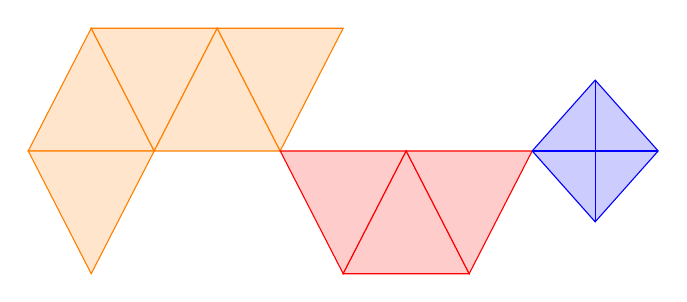
\begin{tikzpicture}[every node/.style={fill,circle,inner sep=1.5pt},yscale=0.9,xscale=0.8]

  % Define the coordinates for the shared vertices of orange triangles
  \coordinate (P1) at (0,0);
  \coordinate (P2) at (2,0);
  \coordinate (P3) at (1,1.732); % height of equilateral triangle
  \coordinate (P4) at (3,1.732);

  % Draw the orange triangles
  \filldraw[orange, fill=orange!20] (P1) -- (P2) -- (P3) -- cycle; % 1st triangle
  \filldraw[orange, fill=orange!20] (P2) -- (P3) -- (P4) -- cycle; % 2nd triangle
  \coordinate (P5) at (4,0); % Shift for the 3rd triangle
  \filldraw[orange, fill=orange!20] (P2) -- (P4) -- (P5) -- cycle; % 3rd triangle
  \coordinate (P6) at (5,1.732); % Height for the 4th triangle
  \filldraw[orange, fill=orange!20] (P4) -- (P5) -- (P6) -- cycle; % 4th triangle
  \coordinate (P7) at (1,-1.732);
  \filldraw[orange, fill=orange!20] (P1) -- (P2) --(P7) -- cycle;

  % Define the coordinates for the red triangles
  \coordinate (R1) at (5,-1.732);
  \coordinate (R2) at (6,0); 
  \coordinate (R3) at (7,-1.732);

  % Draw the red triangles
  \filldraw[red, fill=red!20] (P5) -- (R1) -- (R2) -- cycle; % 1st red triangle
  \filldraw[red, fill=red!20] (R2) -- (R1) -- (R3) -- cycle; % 2nd red triangle

  % The 3rd red triangle
  \coordinate (R4) at (8,0);
  \filldraw[red, fill=red!20] (R2) -- (R3) -- (R4) -- cycle;

  % Draw the 4-clique to the right
  \coordinate (C1) at (8,0); % Shared with 3rd red triangle
  \coordinate (C2) at (9,1);
  \coordinate (C3) at (9,-1);
  \coordinate (C4) at (10,0);
  \filldraw[blue, fill=blue!20] (R4) -- (C1) -- (C2) -- (C4) -- (C3) -- (C1); % Edges of 4-clique
  \draw[blue] (C2) -- (C3); % Diagonal of 4-clique
  \draw[blue] (C4) -- (C1); % Connect 3rd red triangle to 4-clique

  % Draw vertices of 4-clique
  % \foreach \i in {1,...,4}{
  %   \fill (C\i) circle [radius=2pt];
  % }
  % \fill (P1) circle [radius=2pt];
  % \fill (P2) circle [radius=2pt];
  % \fill (P3) circle [radius=2pt];
  % \fill (P4) circle [radius=2pt];
  % \fill (P5) circle [radius=2pt];
  % \fill (P6) circle [radius=2pt];
  % \fill (R1) circle [radius=2pt];
  % \fill (R2) circle [radius=2pt];
  % \fill (R3) circle [radius=2pt];
  % \fill (R4) circle [radius=2pt];
  % \fill (R5) circle [radius=2pt];
  
\end{tikzpicture}
         \caption{An example of hypergraph $H$. Triangles filled with colors represent hyperedges in $\hG$. Two hyperedges are 2-connected if they share two nodes. Different 2-connected components are marked in different colors. }
\label{fig:2-connectivity-H}
% \vspace{12mm}
\end{minipage}%
\hfill
\begin{minipage}{.45\textwidth}
\centering
   % \resizebox{0.7\textwidth}{!}{
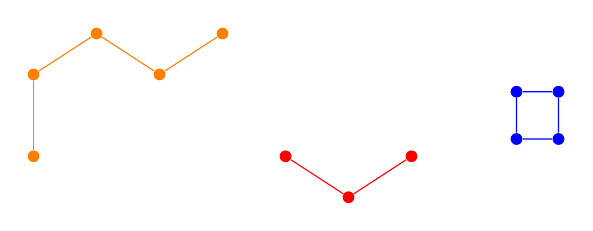
\begin{tikzpicture}[,yscale=0.9,xscale=0.8]
  % Nodes
    % Define the coordinates for the shared vertices of orange triangles
  \coordinate (P1) at (0,0);
  \coordinate (P2) at (2,0);
  \coordinate (P3) at (1,1.732); % height of equilateral triangle
  \coordinate (P4) at (3,1.732);
  \coordinate (P5) at (4,0);
  \coordinate (P6) at (5,1.732);
  \coordinate (P7) at (1,-1.732);

    % Define the coordinates for the red triangles
  \coordinate (R1) at (5,-1.732);
  \coordinate (R2) at (6,0); 
  \coordinate (R3) at (7,-1.732);

    % Draw the 4-clique to the right
  \coordinate (C1) at (8,0); % Shared with 3rd red triangle
  \coordinate (C2) at (9,1);
  \coordinate (C3) at (9,-1);
  \coordinate (C4) at (10,0);
  \coordinate (C5) at (9,0);

  \node (b1) at (barycentric cs:P1=1,P2=1,P3=1) [circle, fill=orange, inner sep=1.5pt] {};
  \node (b2) at (barycentric cs:P2=1,P3=1,P4=1) [circle, fill=orange, inner sep=1.5pt] {};
  \node (b3) at (barycentric cs:P2=1,P4=1,P5=1) [circle, fill=orange, inner sep=1.5pt] {};
  \node (b4) at (barycentric cs:P4=1,P5=1,P6=1) [circle, fill=orange, inner sep=1.5pt] {};
  \node (b5) at (barycentric cs:P1=1,P2=1,P7=1) [circle, fill=orange, inner sep=1.5pt] {};

  % Draw lines between adjacent orange barycenters
  \draw[orange] (b1) -- (b2);
  \draw[orange] (b2) -- (b3);
  \draw[orange] (b3) -- (b4);
  \draw[orange] (b1) -- (b5);

  \node (br1) at (barycentric cs:P5=1,R1=1,R2=1) [circle, fill=red, inner sep=1.5pt] {};
  \node (br2) at (barycentric cs:R2=1,R1=1,R3=1) [circle, fill=red, inner sep=1.5pt] {};
  \node (br3) at (barycentric cs:R2=1,R3=1,C1=1) [circle, fill=red, inner sep=1.5pt] {};
  \draw[red] (br1) -- (br2) -- (br3);

    \node (bc1) at (barycentric cs:C1=1,C2=1,C5=1) [circle, fill=blue, inner sep=1.5pt] {};
  \node (bc2) at (barycentric cs:C2=1,C4=1,C5=1) [circle, fill=blue, inner sep=1.5pt] {};
  \node (bc3) at (barycentric cs:C3=1,C4=1,C5=1) [circle, fill=blue, inner sep=1.5pt] {};
  \node (bc4) at (barycentric cs:C3=1,C1=1,C5=1) [circle, fill=blue, inner sep=1.5pt] {};
  \draw[blue] (bc1) -- (bc2) -- (bc3) -- (bc4) -- (bc1);
\end{tikzpicture}
         \caption{The corresponding graph $\cG_H$. Each node in $\cG_H$ corresponds to a hyperedge in $H$. Two nodes are connected if their corresponding hyperedges share two nodes.}
         % \label{fig:three sin x}
     % \end{subfigure}
% \caption{An example of  2-connectivity and 2-connected components when $d=3$.}
\label{fig:2-connectivity-G}
\end{minipage}
\end{figure}

\begin{figure}
     \centering
     \begin{subfigure}[t]{0.48\textwidth}
         \centering
         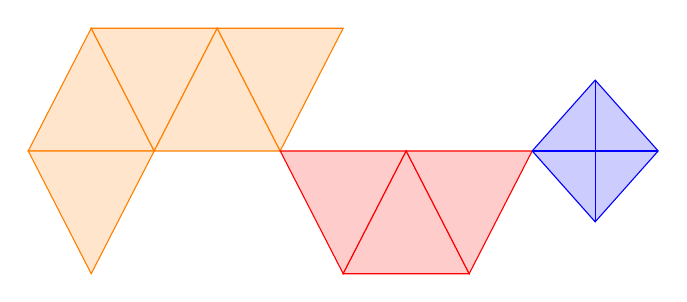
\begin{tikzpicture}[every node/.style={fill,circle,inner sep=1.5pt},yscale=0.9,xscale=0.8]

  % Define the coordinates for the shared vertices of orange triangles
  \coordinate (P1) at (0,0);
  \coordinate (P2) at (2,0);
  \coordinate (P3) at (1,1.732); % height of equilateral triangle
  \coordinate (P4) at (3,1.732);

  % Draw the orange triangles
  \filldraw[orange, fill=orange!20] (P1) -- (P2) -- (P3) -- cycle; % 1st triangle
  \filldraw[orange, fill=orange!20] (P2) -- (P3) -- (P4) -- cycle; % 2nd triangle
  \coordinate (P5) at (4,0); % Shift for the 3rd triangle
  \filldraw[orange, fill=orange!20] (P2) -- (P4) -- (P5) -- cycle; % 3rd triangle
  \coordinate (P6) at (5,1.732); % Height for the 4th triangle
  \filldraw[orange, fill=orange!20] (P4) -- (P5) -- (P6) -- cycle; % 4th triangle
  \coordinate (P7) at (1,-1.732);
  \filldraw[orange, fill=orange!20] (P1) -- (P2) --(P7) -- cycle;

  % Define the coordinates for the red triangles
  \coordinate (R1) at (5,-1.732);
  \coordinate (R2) at (6,0); 
  \coordinate (R3) at (7,-1.732);

  % Draw the red triangles
  \filldraw[red, fill=red!20] (P5) -- (R1) -- (R2) -- cycle; % 1st red triangle
  \filldraw[red, fill=red!20] (R2) -- (R1) -- (R3) -- cycle; % 2nd red triangle

  % The 3rd red triangle
  \coordinate (R4) at (8,0);
  \filldraw[red, fill=red!20] (R2) -- (R3) -- (R4) -- cycle;

  % Draw the 4-clique to the right
  \coordinate (C1) at (8,0); % Shared with 3rd red triangle
  \coordinate (C2) at (9,1);
  \coordinate (C3) at (9,-1);
  \coordinate (C4) at (10,0);
  \filldraw[blue, fill=blue!20] (R4) -- (C1) -- (C2) -- (C4) -- (C3) -- (C1); % Edges of 4-clique
  \draw[blue] (C2) -- (C3); % Diagonal of 4-clique
  \draw[blue] (C4) -- (C1); % Connect 3rd red triangle to 4-clique

  % Draw vertices of 4-clique
  % \foreach \i in {1,...,4}{
  %   \fill (C\i) circle [radius=2pt];
  % }
  % \fill (P1) circle [radius=2pt];
  % \fill (P2) circle [radius=2pt];
  % \fill (P3) circle [radius=2pt];
  % \fill (P4) circle [radius=2pt];
  % \fill (P5) circle [radius=2pt];
  % \fill (P6) circle [radius=2pt];
  % \fill (R1) circle [radius=2pt];
  % \fill (R2) circle [radius=2pt];
  % \fill (R3) circle [radius=2pt];
  % \fill (R4) circle [radius=2pt];
  % \fill (R5) circle [radius=2pt];
  
\end{tikzpicture}
         \caption{An example of hypergraph $H$. Triangles filled with colors represent hyperedges in $\hG$. Two hyperedges are 2-connected if they share two nodes. Different 2-connected components are marked in different colors. }
     \end{subfigure}
     \hfill
     \begin{subfigure}[t]{0.48\textwidth}
         \centering
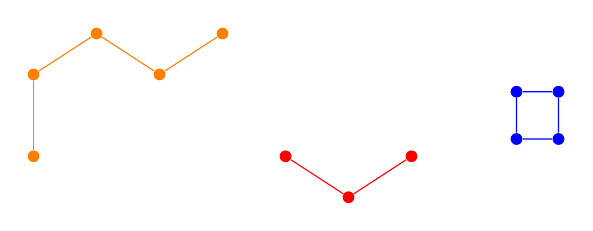
\begin{tikzpicture}[,yscale=0.9,xscale=0.8]
  % Nodes
    % Define the coordinates for the shared vertices of orange triangles
  \coordinate (P1) at (0,0);
  \coordinate (P2) at (2,0);
  \coordinate (P3) at (1,1.732); % height of equilateral triangle
  \coordinate (P4) at (3,1.732);
  \coordinate (P5) at (4,0);
  \coordinate (P6) at (5,1.732);
  \coordinate (P7) at (1,-1.732);

    % Define the coordinates for the red triangles
  \coordinate (R1) at (5,-1.732);
  \coordinate (R2) at (6,0); 
  \coordinate (R3) at (7,-1.732);

    % Draw the 4-clique to the right
  \coordinate (C1) at (8,0); % Shared with 3rd red triangle
  \coordinate (C2) at (9,1);
  \coordinate (C3) at (9,-1);
  \coordinate (C4) at (10,0);
  \coordinate (C5) at (9,0);

  \node (b1) at (barycentric cs:P1=1,P2=1,P3=1) [circle, fill=orange, inner sep=1.5pt] {};
  \node (b2) at (barycentric cs:P2=1,P3=1,P4=1) [circle, fill=orange, inner sep=1.5pt] {};
  \node (b3) at (barycentric cs:P2=1,P4=1,P5=1) [circle, fill=orange, inner sep=1.5pt] {};
  \node (b4) at (barycentric cs:P4=1,P5=1,P6=1) [circle, fill=orange, inner sep=1.5pt] {};
  \node (b5) at (barycentric cs:P1=1,P2=1,P7=1) [circle, fill=orange, inner sep=1.5pt] {};

  % Draw lines between adjacent orange barycenters
  \draw[orange] (b1) -- (b2);
  \draw[orange] (b2) -- (b3);
  \draw[orange] (b3) -- (b4);
  \draw[orange] (b1) -- (b5);

  \node (br1) at (barycentric cs:P5=1,R1=1,R2=1) [circle, fill=red, inner sep=1.5pt] {};
  \node (br2) at (barycentric cs:R2=1,R1=1,R3=1) [circle, fill=red, inner sep=1.5pt] {};
  \node (br3) at (barycentric cs:R2=1,R3=1,C1=1) [circle, fill=red, inner sep=1.5pt] {};
  \draw[red] (br1) -- (br2) -- (br3);

    \node (bc1) at (barycentric cs:C1=1,C2=1,C5=1) [circle, fill=blue, inner sep=1.5pt] {};
  \node (bc2) at (barycentric cs:C2=1,C4=1,C5=1) [circle, fill=blue, inner sep=1.5pt] {};
  \node (bc3) at (barycentric cs:C3=1,C4=1,C5=1) [circle, fill=blue, inner sep=1.5pt] {};
  \node (bc4) at (barycentric cs:C3=1,C1=1,C5=1) [circle, fill=blue, inner sep=1.5pt] {};
  \draw[blue] (bc1) -- (bc2) -- (bc3) -- (bc4) -- (bc1);
\end{tikzpicture}
         \caption{The corresponding graph $\cG_H$. Each node in $\cG_H$ corresponds to a hyperedge in $H$. Two nodes are connected if their corresponding hyperedges share two nodes.}
         \label{fig:three sin x}
     \end{subfigure}
\caption{An example of  2-connectivity and 2-connected components when $d=3$.}
\label{fig:2-connectivity}
\end{figure}


\subsubsection{Decomposition of MAP Across 2-Connected Components}

The following lemma implies that the task of finding the minimum preimage \emph{decomposes} and can be carried out individually in each of the 2-connected components of hyperedges. 


Recall that the clique hypergraph $\cliG$ (defined at the start of Section~\ref{sec:maxclique}) of a graph $G=(V,E)$ has hyperedge set $\cli(E) = \b\{\he\in \textstyle{\binom{[n]}{d}} : (i,j)\in E
\text{ for every } \{i,j\}\subset h
\b\}$.

\begin{lemma}\label{lem:union-min-preimage}
Let $C_1,\cdots, C_m$ be all 2-connected components (i.e., 2-connected subsets of hyperedges) of the clique hypergraph $\cliG$ of the projected graph $G_p=([n],E_p)$. We have
\[
\prim(\pG) = \{\cup_{i=1}^m\hG_i: \hG_i\in \prim(\proj(C_i))\}.
\]
In words, any preimage of $\pG$ is given by a union of hypergraphs, each from a preimage of the projection of a 2-connected component of $\cliG$.
% We abuse notation and use $\proj^{-1}(H)$ to denote $\proj^{-1}(\proj(H))$. 
    % The set of preimages of $\pG$ is given by the union of the preimages of \nbyp{projections of} every 2-connected component of $\cliG$.

    % \nbyp{This is really poorly phrased, because what you mean is that you have to select different preimages for different components. Just remove the statement of the Lemma and make the statement be the first paragraph (including the display) of the proof.}
\end{lemma}
The proof of the lemma is given in Appendix~\ref{sec:union-min-preimage}. 
% \red{YP: don't you want to say instead that the pre-image is given by a Cartesian product of pre-images of components?}\cg{CG: I think we need to say that it is the union of the preimages of components, not just a tuple of preimages}

What makes this decomposition so useful is that with high probability each of the components is of constant size. This will allow us to carry out a brute-force search on each component. 

\begin{restatable}{lemma}{component}\label{lem:component-constant-size}
     For any fixed $\delta<\frac{d-1}{d+1}
     % =:\tcth
     $, with high probability, all 2-connected components of $\cliG$ have size at most $1+2^{d+1}/(\frac{d-1}{d+1}-\delta)=O_n(1)$.
\end{restatable}
% \cg{Give a name for the threshold and add an illustration.}

% \red{
We will refer to this threshold, $\tcth$, as the \emph{\cth}. 
% It will play an important role in our analysis.
% }
% \cg{We didn't prove 2-connectivity of the entire graph above the threshold, so the name might be misleading.}

\subsubsection{MAP Algorithm}
% In the next section, we will show that when $\delta<\frac{d-1}{d+1}$, with high probability all 2-connected components are of constant size. This gives us 
We have the following efficient algorithm that (with high probability) implements the MAP rule $\cA^*$:
\begin{algorithm}\caption{Maximum a Posteriori (MAP) $\cA^*$}\label{alg:map}
\begin{algorithmic}[1]
\State Input: $\pG = ([n],\pE)$
\State Calculate the clique graph $\cliG$ from $\pG$ by finding all size-$d$ cliques in $\pG$.
\State Enumerate over all pairs of vertices to determine 2-neighborhoods of all hyperedges in $\cliG$.
\State Find all 2-connected components of $\cliG$ using a depth-first search on all hyperedges in $\cliG$.
\State Search over all preimages in each 2-connected components of $\cliG$ and find one with minimum size. 
\State Output the union of the minimum preimages of the 2-connected components in $\cliG$.
\end{algorithmic}
\end{algorithm}

% \begin{algorithm}\caption{Maximum a Posteriori (MAP) $\cA^*$}\label{alg:map}
% \begin{algorithmic}[1]
% \STATE Input: $\pG = ([n],\pE)$.
% \STATE Calculate the clique graph $\cliG$ from $\pG$ by finding all size-$d$ cliques in $\pG$.
% \STATE Enumerate over all pairs of vertices to determine 2-neighborhoods of all hyperedges in $\cliG$.
% \STATE Find all 2-connected components of $\cliG$ using depth first search on all hyperedges in $\cliG$.
% \STATE Search over all preimages in each 2-connected components of $\cliG$ and find one with minimum size. 
% \STATE Output the union of minimum preimages of all 2-connected components in $\cliG$.
% \end{algorithmic}
% \end{algorithm}

% This gives us an efficient algorithm for MAP.

\begin{proof}[Proof of Theorem~\ref{thm:sparse-algo}]
From the previous section, we know that MAP returns an arbitrary minimum preimage of the projected graph $\pG$. By Lemma~\ref{lem:union-min-preimage}, a minimum preimage of $\pG$ is given by the union of minimum preimages of all 2-connected components in $\cliG$. So Algorithnm~\ref{alg:map} indeed implements the MAP rule.

% This gives us the following procedure of calculating MAP:
% \begin{enumerate}
%     \item Calculate the clique graph $\cliG$ from $\pG$ by finding all size-$d$ cliques in $\pG$.
%     \item Find all 2-connected components of $\cliG$ by union-find algorithm.
%     \item Search over all possible preimages in each 2-connected components of $\cliG$ and find the one with minimum size. 
%     \item Output the union of minimum preimages of all 2-connected components in $\cliG$.
% \end{enumerate}
We now analyze the running time of the algorithm. Steps 2 and 4 take time at most $O_n(n^d)$. Step 3 takes time at most $O_n(n^2)$. 
Step 5 takes time at most $n^d2^k$, where $k$ is the size of the largest 2-connected component in $\cliG$. By Lemma~\ref{lem:component-constant-size}, $k=O_n(1)$ with high probability, so overall the algorithm finishes in time $O_n(n^d)$ with high probability.
% \cg{If we are careful about how the hyperedges are represented, and use list instead of a tensor, we can improve the running time to be $f(d)n^{g(\delta)}\le f(d)n^{3}$. This requires an extra bound on the number of inclusions. Not sure if this worth writing up. Maybe put in the appendix}\cg{Maybe mention that time complexity blows up when $\delta$ approaches the branching threshold}
\end{proof}

\subsubsection{2-Connected Components have Constant Size for Sparse Hypergraphs}\label{sec:const-size}
In this section we give a proof sketch of Lemma~\ref{lem:component-constant-size} which states that $\cliG$ can be partitioned into small 2-connected components for $\delta$ below $\frac{d-1}{d+1}$. 
We give the full proof in Section~\ref{sec:growth-components}.


The lemma is proved by carefully examining how a set of 2-connected edges in $\cliG$ can grow bigger. This is analogous to (but  more delicate than) the analysis of components in subcritical Erd\H os-R\'enyi graphs.  We will show that any 2-connected component can be decomposed into a series of ``growth'' steps starting from a single hyperedge. Each growth operation has a ``probabilistic cost" because it is a moderately low probability event, which reduces the number of such components. Accounting for the possible growth patterns within 2-connected components in $\cliG$ shows that with high probability no large components appear. 

Now let us consider the possible ways to grow a sub-hypergraph $\shG\subset \rhG$ via local exploration, and try to understand why the probability of having the graph in $\cliG$ decreases with the growth. Suppose $\shG$ is a set of hyperedges, and $\cli(\proj(\shG))$ is 2-connected. For $\shG$ to get larger, it must include one of its 2-neighbors $\he\in \cliG$. How did $\he$ appear in $\cliG$? The somewhat delicate aspect of this is that $\he$ may not be in $\rhG$: $\he$ might exist in $\cliG$ because all edges in the clique $\proj(\he)$ are covered by \emph{some other} hyperedges $\hE\subset \rhG$. So to grow $\shG$, one option is to include all of $\hE$. 
Because each hyperedge is included with fairly small probability, this reduces the expected number of components of the given form, while the number of options in selecting $\hE$ increases with the size of $\hE$. The following lemma gives
the expected number of appearances of a given sub-hypergraph $\shG$ in terms of the number of nodes and the number of hyperedges in the sub-hypergraph.  

% \cg{Should we put the definition of grow here? It's also needed later in the description of the algorithm. We can make more precise claims but the definition is very complicated.}

% Lemma~\ref{lem:number-appearance} states that 

\begin{lemma}\label{lem:number-appearance} Let $X_{\shG}$ be the number of appearances of a sub-hypergraph $\shG$ in $\rhG$. Denote by $v_\shG$ and $e_\shG$ the number of nodes and hyperedges in $\shG$.
    For any hypergraph $\shG$, 
    \[
    \E X_{\shG} = \Theta_n(n^{v_\shG}p^{e_\shG})\,.
    \]
\end{lemma}
When we grow $\shG$, we increase both the number of nodes and the number of edges of the hypergraph. With more nodes, the expectation increases (more possible choices) and with more hyperedges, the expectation decreases. The trade-off is controlled by how we choose $\hE$ and the parameter $\delta$. When $\delta<\frac{d-1}{d+1}$, we will be able to show that no matter how $\hE$ is chosen, the expectation always decreases by a polynomial factor. Therefore, after a constant number of growth steps, the expectation becomes negligible.

% \cg{Here $H$ (and ambiguous graph in the next section) refers to a copy of a sub-hypergraph, so the vertex set is not on $[n]$ but on a small number of vertices in a different space. Do we want a separate notation for subgraphs and sub-hypergraphs? Also strictly we should say the number of subgraphs in $\rhG$ that is isomorphic to $H$ instead of the number of appearances of sub-hypergraph $H$.}

% \cg{
% I think right now the statement is intuitive, as $H$ do serve as possible sub-hypergraphs. But technically it is not a specific sub-hypergraph but refers to all possible copies.}
\subsection{Ambiguous Graphs and Success Probability of MAP}
In this section, we will see that when $\delta $ is below the \cth\  $\tcth$, the success probability of MAP is fully determined by graphs with non-unique minimum preimages, which we call ambiguous graphs.

\begin{definition}\label{def:ambiguous}
    An \emph{ambiguous graph} is a graph with at least two minimum hypergraph preimages.
\end{definition}


As we will see, appearance or non-appearance of ambiguous graphs determines success of the MAP rule. 

\subsubsection{Impossibility Result via Existence 
 of Ambiguous Graphs}
 
In the previous section, we showed that MAP is w.h.p. efficient whenever $\delta<\frac{d-1}{d+1}$. However, even the optimal algorithm does not always succeed in this regime. Consider the graph depicted in Figure~\ref{fig:ambiguous-graph}. If $\pG$ has a copy of this graph as a component, then there are two minimum preimages with equal size, both with the same posterior probability. So no matter which one the MAP algorithm outputs, it must incur at least 1/2 probability of error. This is formalized in the following lemma.


\begin{figure}

   \begin{minipage}{0.48\textwidth}\centering
   % \resizebox{0.45\textwidth}{!}{
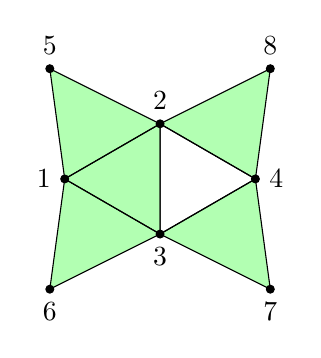
\begin{tikzpicture}[node/.style={minimum size = 1mm, inner sep=0pt}, scale=0.7]
    % Define vertices of the triangles
    \coordinate (1) at (-1.73,0);
    \coordinate (2) at (0,1);
    \coordinate (3) at (0,-1);
    \coordinate (4) at (1.73,0);
    \coordinate (5) at (-2,2);
    \coordinate (6) at (-2,-2);
    \coordinate (7) at (2,-2);
    \coordinate (8) at (2,2);

    
    \fill[green!30] (1) -- (2) -- (3) -- cycle;
    \fill[green!30] (1) -- (2) -- (5) -- cycle;
    \fill[green!30] (1) -- (3) -- (6) -- cycle;
    \fill[green!30] (4) -- (2) -- (8) -- cycle;
    \fill[green!30] (4) -- (7) -- (3) -- cycle;

    % Draw triangles
    \draw (1) -- (2) -- (3) -- cycle;
    \draw (2) -- (3) -- (4) -- cycle;
    \draw (1) -- (2) -- (5) -- cycle;
    \draw (1) -- (3) -- (6) -- cycle;
    \draw (2) -- (4) -- (8) -- cycle;
    \draw (3) -- (4) -- (7) -- cycle;

    % Label vertices
    \node at (1) [draw, circle, fill=black, scale=0.5,inner sep=2pt, label=left:1] {};
    \node at (2) [draw, circle, fill=black, scale=0.5,inner sep=2pt, label=above:2] {};
    \node at (3) [draw, circle, fill=black, scale=0.5,inner sep=2pt, label=below:3] {};
    \node at (4) [draw, circle, fill=black, scale=0.5,inner sep=2pt, label=right:4] {};
    \node at (5) [draw, circle, fill=black, scale=0.5,inner sep=2pt, label=above:5] {};
    \node at (6) [draw, circle, fill=black,scale=0.5, inner sep=2pt, label=below:6] {};
    \node at (7) [draw, circle, fill=black, scale=0.5,inner sep=2pt, label=below:7] {};
    \node at (8) [draw, circle, fill=black, scale=0.5,inner sep=2pt, label=above:8] {};

\end{tikzpicture}
    % \caption{A graph with non-unique minimum preimage when $d=3$. Green hyperedges are the two possible minimum preimages.}
    % \label{fig:ambiguous-graph}
% \end{figure}
\end{minipage}\hfill
   \begin{minipage}{0.48\textwidth}\centering

% \begin{figure}
% \centering
% % \begin{subfigure}{}
% % \end{subfigure}
% % \hfill
% \begin{subfigure}
% \centering
   % \resizebox{0.45\textwidth}{!}{
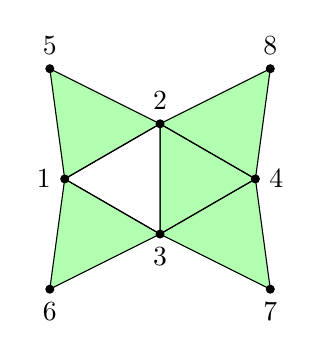
\begin{tikzpicture}[node/.style={minimum size = 0mm, inner sep=0pt}, scale=0.7]
    % Define vertices of the triangles
    \coordinate (1) at (-1.73,0);
    \coordinate (2) at (0,1);
    \coordinate (3) at (0,-1);
    \coordinate (4) at (1.73,0);
    \coordinate (5) at (-2,2);
    \coordinate (6) at (-2,-2);
    \coordinate (7) at (2,-2);
    \coordinate (8) at (2,2);

    
    \fill[green!30] (4) -- (2) -- (3) -- cycle;
    \fill[green!30] (1) -- (2) -- (5) -- cycle;
    \fill[green!30] (1) -- (3) -- (6) -- cycle;
    \fill[green!30] (4) -- (2) -- (8) -- cycle;
    \fill[green!30] (4) -- (7) -- (3) -- cycle;

    % Draw triangles
    \draw (1) -- (2) -- (3) -- cycle;
    \draw (2) -- (3) -- (4) -- cycle;
    \draw (1) -- (2) -- (5) -- cycle;
    \draw (1) -- (3) -- (6) -- cycle;
    \draw (2) -- (4) -- (8) -- cycle;
    \draw (3) -- (4) -- (7) -- cycle;

    % Label vertices
    \node at (1) [draw, circle, fill=black,scale=0.5, inner sep=2pt, label=left:1] {};
    \node at (2) [draw, circle, fill=black,scale=0.5, inner sep=2pt, label=above:2] {};
    \node at (3) [draw, circle, fill=black,scale=0.5, inner sep=2pt, label=below:3] {};
    \node at (4) [draw, circle, fill=black,scale=0.5, inner sep=2pt, label=right:4] {};
    \node at (5) [draw, circle, fill=black,scale=0.5, inner sep=2pt, label=above:5] {};
    \node at (6) [draw, circle, fill=black,scale=0.5, inner sep=2pt, label=below:6] {};
    \node at (7) [draw, circle, fill=black,scale=0.5, inner sep=2pt, label=below:7] {};
    \node at (8) [draw, circle, fill=black,scale=0.5, inner sep=2pt, label=above:8] {};

\end{tikzpicture}
% }
% \end{subfigure}

\end{minipage}
\caption{A graph with non-unique minimum preimage in the case $d=3$. The green hyperedges are the two possible minimum preimages.}
\label{fig:ambiguous-graph}
\end{figure}

\begin{restatable}{lemma}{badgraphinisolation}\label{lem:bad-graph-in-isolation}
    For any ambiguous graph $G_a$ and any recovery algorithm $\cA$, given input $\pG = \proj(\rhG)$,
    \[
    \Pr(\cA(\pG)\ne\rhG) \ge \frac{1}{2}\Pr\b(\cli(G_a)\text{ is a 2-connected component of }\cliG \b)\,.
    \]
\end{restatable}

% \begin{lemma}\label{lem:bad-graph-in-isolation}

% \end{lemma}
\begin{proof}
By Lemma~\ref{lem:union-min-preimage}, a minimum preimage of $\pG$ is given by the union of the minimum preimages of every 2-connected component of $\cliG$. Therefore, when $\cli(G_a)$ is a 2-connected component of $\cliG$, the minimum preimage of $\cliG$ is not unique. So no matter which hypergraph $\cA^*$ chooses, it has at least 1/2 probability of making a mistake. In other words,
\[
\Pr(\cA(\pG)\ne\rhG|\cli(G_a)\text{ is a 2-connected component of }\cliG) \ge 1/2\,.
\]
The lemma follows from Bayes rule. 
\end{proof}

It follows that to prove impossibility of (exact) recovery, we only need to find an ambiguous graph that is a 2-connected component with probability $\Omega_n(1)$.
% \cg{Define ambiguous graph threshold}
Let the \emph{ambiguity threshold}, $\ath$, be the infimum of $\delta$ such that there exists an ambiguous graph appearing as a 2-connected component with probability $\Omega_n(1).$
\[
\ath \defeq \inf\{\delta:\exists G_a, \Pr(\cli(G_a)\text{ is a 2-connected component of }\cliG) = \Omega_n(1) \}\,.
\]
It then follows from Lemma~\ref{lem:bad-graph-in-isolation} that exact recovery is impossible for any $\delta$ that is at least $\ath$. 
% In other words, $\cdel d \le \ath$.
% \red{
In other words, we have the following corollary.
\begin{corollary}\label{cor:critical-threshold-smaller-ambiguous-threshold}
    For any $d$, we have $\cdel d \le \ath\,.$
\end{corollary}
% }


This will allow us to prove the impossibility results in Theorem~\ref{thm:main-three} and Theorem~\ref{thm:main-four-five} showing that $\ath$, and hence also $\cdel d$, is at most $\frac{2d-4}{2d-1}$ when $d\le 5$.  The construction of the ambiguous graph will be described in Section~\ref{sec:impossibility}. It will be a generalization of Figure~\ref{fig:ambiguous-graph} to general $d$.


This approach stops working for $d\ge 6$. In Section~\ref{sec:impossibility}, we will show that the regime of $\delta$ in which such an ambiguous graph appears as a 2-connected component in $\rhG$ is between $\frac{2d-4}{2d-1}$ and the \cth\ $\frac{d-1}{d+1}$. When $d\ge 6$, $\frac{2d-4}{2d-1}$ is above the \cth\ and the ambiguous graph typically overlaps with other hyperedges, i.e., it does not appear as a component. In this case it is no longer clear that there are at least two equally likely preimages.

We next work towards understanding
when a given sub-hypergraph will appear in $\rhG$.

\subsubsection{Appearance of Sub-hypergraphs in Random Hypergraphs}

We will need a lemma that determines the threshold density for a given graph to appear in the random $d$-hypergraph, $\rhG(n,d,p)$.
The graph version of the lemma was first proven in \cite{bollobas1981threshold} and simplified in \cite{rucinski1986strongly}. For random hypergraphs, the proof is similar and we include it in Appendix~\ref{sec:subgraph_threshold} for completeness.
\begin{lemma}\label{lem:subgraph_threshold}
    For a hypergraph $\shG = (V,\hE_\shG)$,
    define \[
    m(\shG) = \max_{\shG'\subset \shG}\frac{e_{\shG'}}{v_{\shG'}}\,,
    \]
    % where $\shG[V']$ is the induced subgraph on $V'$ and $e$ denotes the number of hyperedges in the subgraph. 
    where $e_{\shG'}$ and $v_{\shG'}$ are the number of edges and the number of nodes of sub-hypergraph $\shG$.
    We have
    \[
    \Pr(\shG\subset \rhG) = 
    \begin{cases}
        o_n(1) &\text{if }p=o_n(n^{-1/m(\shG)})\\
        1-o_n(1) &\text{if }p=\omega_n(n^{-1/m(\shG)})\\
        \Omega_n(1) &\text{if } p =\Theta_n(n^{-1/m(\shG)}).
    \end{cases}
    \]
\end{lemma}


\subsubsection{Reconstruction Result by Nonexistence of Ambiguous Graphs}\label{sec:main-idea-reconstruction}
In this section we prove the following theorem.
\begin{theorem}\label{thm:delta-lower}
    When $d=3$ and $\delta<2/5$ or when $d=4,5$ and $\delta<1/2$, the MAP rule achieves exact recovery and moreover it can be implemented efficiently.
\end{theorem}
In the regime where $\delta<
% \tcth=
\frac{d-1}{d+1}$, which is the regime we care about when $d\le 5$, the converse of Lemma~\ref{lem:bad-graph-in-isolation} is also true. That is, if with high probability no ambiguous graph (i.e., with non-unique minimum cover) appears in $\pG$ as a 2-connected component, then MAP succeeds with high probability.

\begin{lemma}\label{lem:no-ambiguous}
    Assume $\delta<
    % \tcth=
    \frac{d-1}{d+1}$.
    If for all finite ambiguous graphs $G_a$,
    \[
    \Pr\b(\cli(G_a)\text{ is a 2-connected component of }\cliG \b)=o_n(1)\,,
    \]
    % $\Pr(G_a\subset \pG)=o_n(1)$
    % with at most $\frac{d(2^d+1)}{\frac{d-1}{d+1}-\delta} $ vertices 
    % with non-unique minimum cover 
    then we have 
    \[
    \Pr(\cA^*(\pG)=\rhG)\ge 1- o_n(1)\,.
    \]
\end{lemma}
% \cg{Define the ambiguous graph threshold. Explain here the relation between the two thresholds.}

The lemma is proved in Appendix~\ref{sec:proof-no-ambiguous}. 
Here we provide a sketch of the proof. If there is no ambiguous graph in $\pG$, the projections of every 2-connected components have a unique minimum preimage. As shown in Lemma~\ref{lem:component-constant-size}, all 2-connected components are of constant size. Under this condition, the minimum preimage of the 2-connected component is correct with probability $1-O_n(p)$, as any other preimage is $O_n(p)$ times less likely in the posterior and there are only constant number of possible preimages. The overall minimum preimage, as given by $\cA^*$, is then correct with high probability by union bound over all 2-connected components.

% \red{
Recall the definition of the ambiguous threshold, $\ath$, Lemma~\ref{lem:no-ambiguous} implies that the critical threshold $\cdel d$ is above $\ath$ if $\ath$ is below $\tcth$.
\begin{corollary}
    For any $d$, if $\ath\le\tcth$, we have $ \cdel d \ge \ath$.
\end{corollary}

Combining this corollary with Corollary~\ref{cor:critical-threshold-smaller-ambiguous-threshold}, we get that the ambiguous threshold $\ath$ fully determines the critical threshold $\cdel d$ if $\ath$ is below $\tcth$.
\begin{corollary}
    For any $d= 3,4,5$, we have $\ath\le\tcth$, and hence $ \cdel d = \ath$.
\end{corollary}
% }
\begin{figure}
    \centering
    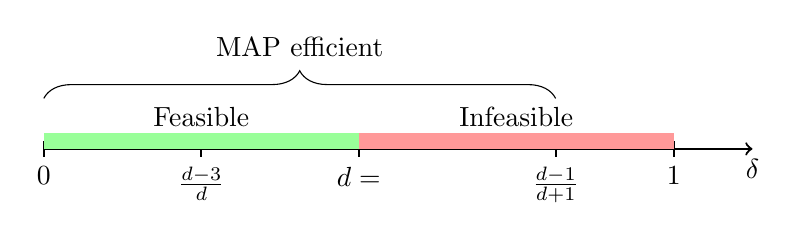
\begin{tikzpicture}
    % Draw the main axis
    \draw[thick, ->] (-4,0) -- (5,0) node[anchor=north] {$\delta$};

    % Draw and label the first threshold
    \draw[thick] ({-2},0.1) -- ({-2},-0.1) node[below] {$\frac{d-3}{d}$};

    % Draw and label the second threshold (ambiguous threshold)
    \draw[thick] (0,0.1) -- (0,-0.1) node[below] {$\cdel d = \ath$};

    % Draw and label the third threshold (2-connectivity threshold)
    \draw[thick] (2.5,0.1) -- (2.5,-0.1) node[below] {$
    % \tcth=
    \frac{d-1}{d+1}$};

    % Add additional ticks and labels as needed
    \foreach \x in {0,1}
        \draw[thick] (8*\x-4,0.1) -- (8*\x-4,-0.1) node[below] {\x};

        % Color the regions
    % Feasible region: from 0 to the ambiguous threshold (green)
    \fill[green!40] (-4,0) rectangle (0.4,0.2);
    \node at (-2,0.4) {Feasible};

    % Infeasible region: from the ambiguous threshold to 1 (red)
    \fill[red!40] (0,0) rectangle (4,0.2);
    \node at (2,0.4) {Infeasible};

    % Add curly brace to indicate region from 0 to 2-connectivity threshold
    \draw [decorate,decoration={brace,amplitude=10pt,raise=4pt},yshift=0pt]
    (-4,0.5) -- (2.5,0.5) node [black,midway,yshift=0.8cm] {MAP efficient};
\end{tikzpicture}
    \caption{
    % \gb{make a second figure with them swapped somehow explaining why for $d\geq 6$ things are different}
    % \red{
    Relation between different thresholds. The maximum clique cover algorithm $\cliA$ succeeds with high probability up to $\delta=\frac{d-3}{d}$. The MAP algorithm is efficient up to $\tcth$ and succeeds with high probability up to threshold $\cdel d$. If $\ath<\tcth$, then $\cdel d$ is the same as the ambiguous threshold $\ath$.
    % }
    }
    \label{fig:thresholds-relation}
\end{figure}

As long as we can check the condition in Lemma~\ref{lem:no-ambiguous} for a specific $\delta$, MAP is optimal. If $\delta<\tcth$, then with high probability all 2-connected components have size bounded by $(2^d+1)/(\frac{d-1}{d+1}-\delta)$, so there are only finitely many graphs we need to check. This gives us the following computer assisted method of proving that MAP works when $\delta $ is below a hypothesized threshold $\delta_0$:
\begin{enumerate}
    \item Enumerate over all hypergraphs $\shG$ with at most $1+2^{d+1}/(\frac{d-1}{d+1}-\delta_0)$ hyperedges.
    \item Compute the probability that $\shG\subset \rhG$ by Lemma~\ref{lem:subgraph_threshold} with $p=n^{-d+1+\delta_0}$.
    % (deferred due to space constraints). 
    \item Enumerate all possible preimages of $\proj(\shG)$ and see if $\proj(\shG)$ is ambiguous.
    \item If all graphs are either not ambiguous or have vanishing probability of occurring, the condition in Lemma~\ref{lem:no-ambiguous} is satisfied and MAP succeeds with high probability at $\delta=\delta_0$.
\end{enumerate}
Since $\Pr(\shG\subset \rhG)$ monotonically increases with $\delta$, we know the same condition holds for any $\delta<\delta_0$.

Although this approach can be carried out in principle, the number of hypergraphs with at most $1+2^{d+1}/(\frac{d-1}{d+1}-\delta_0)$ hyperedges is a huge number and cannot be verified in reasonable time. Instead of doing a brute force search, we will utilize the structure of how 2-connected components grow, as discussed in Section~\ref{sec:const-size}, to reduce the runtime. The runtime of the search can be further reduced by identifying properties of ambiguous graph and focusing on graphs with such properties. 

With the computer search, we are able to prove the following lemma. The search algorithm will be discussed in more detail in Section~\ref{sec:algo-proof}.
\begin{restatable}{lemma}{lowerbound}\label{lem:delta-lowerbound}
    When $d=3$ and $\delta<2/5$ or when $d=4,5$ and $\delta<1/2$, any ambiguous graph $G_a$ 
    % of size at most $2\binom{d}{2}/\b({\frac{d-1}{d+1}-\delta} \b)$
    satisfies
    $
    \Pr(G_a\subset \pG)=o_n(1).
    $
\end{restatable}

Combining this lemma and Lemma~\ref{lem:no-ambiguous} completes the proof of Theorem~\ref{thm:delta-lower}.
% \begin{proof}[proof of Theorem~\ref{thm:delta-lower}]
% Follows directly from Lemma~\ref{lem:no-ambiguous} and Lemma~\ref{lem:delta-lowerbound}.
% \end{proof}
\subsection{Upper Bound on $\cdel d$ for Large $d$ and Proof of Theorem~\ref{thm:main-large-d}}
We identify a sufficient condition for the (optimal) MAP rule to fail:
Suppose there is a hyperedge $\he$ in $\rhG$ where every pair of nodes in $\he$ is also included in other hyperedges in $\rhG$. In this case the graph $\rhG\setminus \{\he\}$ has higher probability and has the same graph projection. 
Because the optimal algorithm outputs a minimum preimage, it does not output the original hypergraph $\rhG$: deleting $\he$ forms a smaller preimage.

We formalize this sufficient condition and consider a hypergraph $\bG$ with the following hyperedges:
\begin{itemize}
    \item $\{v_1,\cdots,v_d\}$,
    \item $\{v_i,v_j,u_{ij}^{(1)}, u_{ij}^{(2)},\cdots, u_{ij}^{(d-2)}\}$ for all $\{i,j\}\subset [d] $, where for each $i$ and $j$ the nodes $u_{ij}^{(1)}, u_{ij}^{(2)},\cdots, u_{ij}^{(d-2)}$ are arbitrary.
\end{itemize}

From the discussion above, we know that $\cA^*$ will fail if $\bG\subset\rhG$, because the hyperedge $v_1,\cdots,v_d$ can be removed from the output and increase the posterior probability. 
% 
Therefore, we have
\[
\Pr(\cA^*(\pG)\ne \rhG) \ge \Pr(\bG\subset\rhG)\,.
\]
By Lemma~\ref{lem:subgraph_threshold}, this occurs with probability $\Omega_n(1)$ when $p=\Omega_n(n^{-1/m(\bG)})$. Since 
\[
m(\bG) = \frac{e_{\bG}}{v_{\bG}} = \frac{\binom{d}{2}+1}{d+\binom{d}{2}(d-2)}\,,
\]
this is equivalent to 
\[
p=\Omega_n(n^{-d\frac{d^2-3d+4}{d^2-d+2}})\,,
\]
or $\delta\ge \frac{d^2-d-2}{d^2-d+2}$.
We have shown the following impossibility result:
\begin{theorem}\label{thm:large-d}
    Exact recovery is information theoretically impossible when  $\delta\ge \frac{d^2-d-2}{d^2-d+2}$\,.
\end{theorem}

% \red{
% \begin{itemize}
%     \item We ask the basic question of when does projecting a hypergraph to a graph losses information, equivalently, when is it possible to recover the original hypergraph from a projected graph.
%     \item Inspiration from social network and biology. How to recover higher order interactions from a graph.
%     \item Some data are inherently hypergraph, but treated as a graph. Examples from social science. 
%     \item We want to understand when is projecting hypergraph to a normal graph a good strategy to develop algorithms. The answer depends on specific question of interest, but we can gain insight by studying the fundamental limit of when the projection start to loss information.
%     \item The same question has been studied from empirical point of view and tested on real data sets.
%     \item To understand the question in theory, we study random hypergraphs, as worst-case hypergraphs is impossible to recover.
%     \item Definition of the problem
%     \item We obtain tight bounds of exact recovery for random $d$-hypergraph when $d=3,4,5$.
%     \item An interval for $d\ge 6$? We can have some simple upper and lower bounds.
%     \item A chart for the results.
% \end{itemize}
% }


